\documentclass{article}
\usepackage[utf8]{inputenc}

%References
\usepackage{hyperref}

%Colors
\usepackage{xcolor}

\usepackage[protrusion=true,expansion]{microtype}

%Code Markup
\usepackage[outputdir=cache]{minted}
%Syntax Highlighting Style
\definecolor{bggray}{RGB}{40,40,40}
\newmintedfile[javacode]{java}{
	style=fruity,
	bgcolor=bggray,
	linenos,
	breaklines
}

%Page Margins and stuff
\usepackage{geometry}
 \geometry{
 a4paper,
 total={170mm,257mm},
 left=20mm,
 }

%Pictures
\usepackage{graphicx}
\graphicspath{ {./images/} }

%Move the title position
\usepackage{titling}

\setlength{\droptitle}{-8.5em} %Up, near the top but not too high

\title{Assignment 2 - Object Oriented Programming}
\author{Daniel Hannon (19484286)}
\date{November 2020}

\begin{document}
	\maketitle
	\section{Overview}

	Within this assignment we have to Define a simple Online Shopping facility as described by the Diagram featured in Lecture 8, among others.\\The function of my Code is fairly straight forward. In order to implement the Shopping Cart I used ArrayList to hold the items as it is more efficient than using a standard array for it has a seach speed of O n comparred to O n squared. \\ For the creation of the various IDs throughout the code I created a private method which utilizes Math.random() as Math.random only returns values between zero and one, I multiply it by an arbitrary number before typecasting the result to long\\ The transaction ID is accompanied by a timestamp which is stored as a string both of which cannot be modified by the end user whatsoever.\\ The Order Class is slightly more complex but still very straightforward. One piece of oversight I made was the ability to make it without the existence of an Address, this is to mimic real life transactions.\\ As a result there is a check before the email is sent to verify the existence of an Address in some capacity. \\ The Address is a dynamic object as it allows for varying amounts of fields, much like a normal address. I created a method Stringify() to merge the address into a formatted string and return it in such a way that it looks nice to the user, this also reduces the amount of get calls that need to be made, hence reducing overall lines of code.\\ Payment records the credit card details and the order details and it validates itself in two ways. It verifies the date is a date and in the correct format, if it is not. Uses the unix Epoch as the substitute date, so it will always fail validation. then it verifies the card type by doing some string compares, and finally it verifies that the number is of adequate length by checking if it is between a certain numeric range, as it is 16-digits, it must be stored as a Long as it is out of the range of the Integer type.
	\section{Code}
	\subsection{TransactionTest}
	\javacode{TestTransaction.java}
	\subsection{ShoppingCart}
	\javacode{ShoppingCart.java}
	\subsection{Order}
	\javacode{Order.java}
	\subsection{Address}
	\javacode{Address.java}
	\subsection{Payment}
	\javacode{Payment.java}
	\newpage
	\subsection{Email}
	\javacode{Email.java}
	\section{Output}
	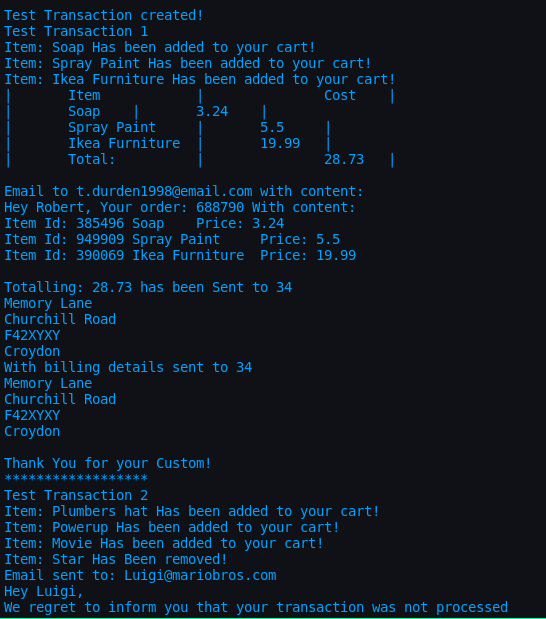
\includegraphics{output.png}
\end{document}